\frame{
	\frametitle{Programa de Trabajo}
%	Para la realización de esta memoria se consideran los siguientes hitos:
%	\begin{center}
%		\begin{tabular}{|l|l|}
%        		\hline
%        		\textbf{Actividad a realizar} & \textbf{Plazo duración} \\
%        		\hline
%			\hline
%	        	Estudiar CUDA & 1 mes \\
%	        	\hline
%        		Estudiar métodos estadísticos predictivos & 1 mes \\
%		        \hline
%		        Diseño de estrategia usando cuda & 1 mes \\
%		        \hline
%		        Implementación & 1 mes \\
%			\hline
%			Medir y evaluar resultados & 1 semana\\
%		        \hline
%	        	Redacción (trabajo constante) & 2 meses\\
%        		\hline
%		\end{tabular}
%	\end{center}
	Para el desarrollo de esta memoria de titulación, se consideraon las siguientes actividades, definiendo sus respectivas duraciones.
        \begin{center}
                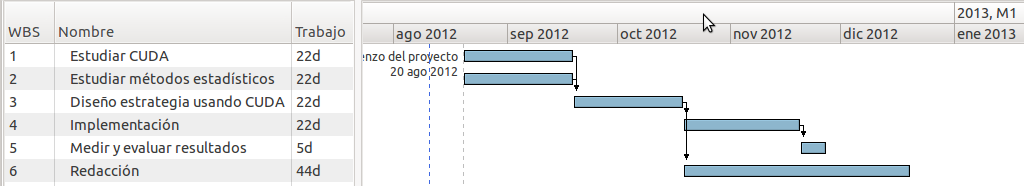
\includegraphics[width=\textwidth]{img/plan}
        \end{center}

}
